\documentclass[fleqn,10pt,twocolumn]{wlscirep}

% Packages
\usepackage{pifont}
\usepackage{amsfonts}
\usepackage{amsmath}
\usepackage{float}
% \usepackage[multiple]{footmisc}
\usepackage{booktabs}
\usepackage{csquotes}
\usepackage{moreverb} % for verbatim ouput (for wordcount)
\usepackage{listings, textcomp}
\lstset{language=Python}

\lstset{ %
  basicstyle=\ttfamily\footnotesize,  % size of fonts used for the code
  xleftmargin=\parindent,
  breaklines=true,   % automatic line breaking only at whitespace
  captionpos=b,   % sets the caption-position to bottom
  commentstyle=\color{gray},  % comment style
  keywordstyle=\color{blue},  % keyword style
  stringstyle=\color{red},  % string literal style
  upquote=true  %straight single quotes (requires textcomp)
}

\usepackage{caption}
\captionsetup{%
   figurename=Fig.,
   tablename=Tab.
}
\usepackage{subcaption}

% New Commands
\newcommand{\cmark}{\ding{51}}%
\newcommand{\xmark}{\ding{55}}%
\newcommand{\code}[1]{\texttt{#1}}
\newcommand{\fixme}[1]{\textcolor{red}{{#1}}}
\newcommand{\inlinecite}[1]{\footnotesize\citen{#1}}
\newcommand{\tightlist}{\setlength{\itemsep}{0pt}\setlength{\parskip}{0pt}}

\usepackage[switch]{lineno}
\linenumbers

\title{NumPy---Array Programming in Python}

\author[1]{Charles R. Harris}
\author[2,3,4,*]{K. Jarrod Millman}
\author[5,2,4,*]{St\'efan J. van der Walt}
\author[6,*]{Ralf Gommers}
\author[7]{Pauli Virtanen}
\author[8]{David Cournapeau}
\author[9]{Eric Wieser}
\author[10]{Julian Taylor}
\author[4]{Sebastian Berg}
\author[11]{Nathaniel J. Smith}
\author[12]{Robert Kern}
\author[4]{Matti Picus}
\author[13]{Stephan Hoyer}
\author[14]{Marten H. van Kerkwijk}
\author[2,15]{Matthew Brett}
\author[16]{Allan Haldane}
\author[17]{Jaime Fern\'andez del R\'io}
\author[18,19]{Mark Wiebe}
\author[6,20,21]{Pearu Peterson}
\author[22,23]{Pierre G\'erard-Marchant}
\author[24]{Kevin Sheppard}
\author[25]{Tyler Reddy}
\author[4]{Warren Weckesser}
\author[6]{Hameer Abbasi}
\author[26]{Christoph Gohlke}
\author[6]{Travis E. Oliphant}
\affil[1]{Independent Researcher, Logan, Utah, USA}
\affil[2]{Helen Wills Neuroscience Institute, University of California, Berkeley, Berkeley, CA, USA}
\affil[3]{Division of Biostatistics, University of California, Berkeley, Berkeley, CA, USA}
\affil[4]{Berkeley Institute for Data Science, University of California, Berkeley, Berkeley, CA, USA}
\affil[5]{Applied Mathematics, Stellenbosch University, Stellenbosch, South Africa}
\affil[6]{Quansight LLC, Austin, TX, USA}
\affil[7]{Department of Physics and Nanoscience Center, University of Jyv\"askyl\"a, Jyv\"askyl\"a, Finland}
\affil[8]{Mercari JP, Tokyo, Japan}
\affil[9]{Department of Engineering, University of Cambridge, Cambridge, UK}
\affil[10]{Independent Researcher, Karlsruhe, Germany}
\affil[11]{Independent Researcher, Berkeley, CA, USA}
\affil[12]{Enthought, Inc., Austin, TX, USA}
\affil[13]{Google Research, Mountain View, CA, USA}
\affil[14]{Department of Astronomy \& Astrophysics, University of Toronto, Toronto, ON, Canada}
\affil[15]{School of Psychology, University of Birmingham, Edgbaston, Birmigham, UK}
\affil[16]{Department of Physics, Temple University, Philadelphia, PA, USA}
\affil[17]{Google, Zurich, Switzerland}
\affil[18]{Department of Physics and Astronomy, The University of British Columbia, Vancouver, BC, Canada}
\affil[19]{Amazon, Seattle, Washington, USA}
\affil[20]{Independent Researcher, Saue, Estonia}
\affil[21]{Department of Mechanics and Applied Mathematics, Institute of Cybernetics at Tallinn Technical University, Tallinn, Estonia}
\affil[22]{Department of Biological and Agricultural Engineering, University of Georgia, Athens, GA}
\affil[23]{France-IX Services, Paris, France}
\affil[24]{Department of Economics, University of Oxford, Oxford, UK}
\affil[25]{CCS-7, Los Alamos National Laboratory, Los Alamos, NM, USA}
\affil[26]{Laboratory for Fluorescence Dynamics, Biomedical Engineering Department, University of California, Irvine, Irvine, CA, USA}
\affil[*]{millman@berkeley.edu, stefanv@berkeley.edu, ralf.gommers@gmail.com}


\keywords{Scientific computing, Python, Mathematics, Array Programming}

\begin{abstract}
% https://www.nature.com/nature/for-authors/formatting-guide

% Articles start with a fully referenced summary paragraph, ideally of no more
% than 200 words, which is separate from the main text and avoids numbers,
% abbreviations, acronyms or measurements unless essential. It is aimed at
% readers outside the discipline.

% This summary paragraph should be structured as follows:
% - 2-3 sentences of basic-level introduction to the field;
% - a brief account of the background and rationale of the work;
% - a statement of the main conclusions (introduced by the phrase 'Here we show' or its equivalent);
% - 2-3 sentences putting the main findings into general context so it is
%   clear how the results described in the paper have moved the field forwards.

% Please refer to our annotated example  to see how the summary paragraph should
% be constructed. https://www.nature.com/documents/nature-summary-paragraph.pdf


% - 2-3 sentences of basic-level introduction to the field;
Array computation libraries provide powerful notation for accessing,
manipulating, and operating on data in vectors, matrices, and
higher-dimensional arrays \cite{iverson1980notation}.
% - a brief account of the background and rationale of the work;
NumPy is the fundamental array computation library for the Python ecosystem
\cite{dubois2007guest,oliphant2007python,millman2011python,perez2011python}.
It has been actively developed for over two decades and has more than 850
contributors, nearly 300,000 dependent repositories on GitHub, and millions of
downloads per year.
It plays an essential role in research analysis pipelines in fields as
diverse as physics, biology, astronomy, neuroscience, material science,
engineering, and chemistry.
For example, in astronomy, NumPy was fundamental to discovering gravitational
waves\cite{pycbc}, the first imaging of a black hole\cite{eht-imaging}, and
continues underpinning the future exploration of our
universe\cite{jenness2018lsst}.
It is one of the most commonly used machine learning tools among
enterprises \cite{451report2018}.
% - a statement of the main conclusions (introduced by the phrase 'Here we show' or its equivalent);
Here we show how a small group of students and scientists created this
popular tool, explain the core ideas that helped make it it successful,
and highlight recent development to better serve new use cases
and future improvements.
% - 2-3 sentences putting the main findings into general context so it is
%   clear how the results described in the paper have moved the field forwards.
NumPy continues to evolve to meet the needs of its community, to remain
relevant in an ever-changing computing landscape, and to be a fundamental
pillar of support for the next decade of scientific computing, data science,
and machine learning in Python.
 
\end{abstract}

\begin{document}

\flushbottom
\maketitle
\thispagestyle{empty}

% Count of words
\verbatiminput{wordcount.tex}

\section{Introduction}

% https://books.google.com/books?id=QQJODwAAQBAJ&pg=PA101&lpg=PA101&dq=%E2%80%9Cthe+secret+to+successful+hiring+is+this:+look+for+the+people+who+want+to+change+the+world.%E2%80%9D&source=bl&ots=D6l8JXfB20&sig=ACfU3U0x1X9Gh8k6MlNV0BqhBa_73Q0yfQ&hl=en&sa=X&ved=2ahUKEwj48pqg_oHgAhVohuAKHYlJAsc4ChDoATAAegQIChAB#v=onepage&q=%E2%80%9Cthe%20secret%20to%20successful%20hiring%20is%20this%3A%20look%20for%20the%20people%20who%20want%20to%20change%20the%20world.%E2%80%9D&f=false
% "The secret to successful hiring is this: look for the people who want to change the world.".  Marc Benioff.

NumPy is both a cause and an effect of a striking shift in the nature of
scientific computing.  The traditional model of scientific software has been of
the user as {\it consumer}.  Writing software is a task for specialists and
professionals, supported by income from selling the software to scientists to
use.  The new model is of the user as {\it owner}.  The Python language, with
the NumPy library, provides a framework that scientists can consume, but has
also been successful in encouraging scientists to develop as programmers, and
to write code for the library, and the system of packages around it.  This has
fostered a new culture of contribution and collaboration in scientific
computing that resulted in a virtuous cycle of increasing use, and increasing
development.

This cycle is one of several explanations for the astonishing growth of NumPy
in scientific computing.

\subsection{History}

The first incarnation of NumPy was a package called Numeric, written in 1995
by Jim Hugunin, then completing his master's thesis at MIT on
superconductor-semiconductor junctions.  Hugunin based his package on previous
work by Jim Fulton, then working at the US Geological Survey, and acknowledges
many others in his initial report of the package \cite{Hugunin-whitepaper}.
Numeric provided an array object in Python, written in C, and linking to
standard fast implementations of linear algebra.

As Hugunin points out, at the time he wrote Numeric, commercial languages for
interactive computing with numerical arrays were already well-established,
including Matlab and IDL.  At the time, it must have seemed a safe bet that
Numeric would not succeed in this market.  The commercial languages were
developed and maintained by large numbers of full-time professional programmers
and supported by formal quality assurance, release managers and writers of
scientific documentation.  In contrast, Numeric, and later, NumPy, would
continue to be developed almost entirely by scientists, including graduate
students and faculty, without specific funding, and often to the detriment of
the scientists' careers.

Table X1 about here: backgrounds of initial designers (mainly math, physics).

Table X2 about here: backgrounds of major committers (mainly math, physics).

Around 1998, the Space Telescope Science Institute (STScI) software group began
to use Python heavily, and, around 2000, wrote a re-implementation of much of
Numeric, called NumArray, to support their need to work on large memory-mapped
arrays, and arrays of mixed data type records \cite{STScI-slither}.  This
briefly caused the Numeric and NumArray communities to diverge, until 2005,
when Travis Oliphant embarked upon a major rewrite that aimed to be a ``best of
both worlds'' unification of Numeric and NumArray \cite{oliphant2006guide}.
This merger resulted in NumPy.  At the time, Oliphant was an assistant
professor of Electrical and Computer Engineering at Brigham Young University.

Over the next 10 years, NumPy attracted a relatively large pool of scientist
developers.  To benefit from these
user-developers, the project developed an increasingly strong culture of using
software-engineering practice to improve collaboration and reduce error
\cite{millman2014developing}. The NumPy team was early in adopting distributed
revision control and code review to improved collaboration on code, and
continuous testing so we run a large battery automated tests for every proposed
change in NumPy. At first, NumPy had rather sparse documentation, but the project
developed a new standard for ``docstrings''---text describing each NumPy
function---and used this standard to write comprehensive high-quality
documentation, integrated with the source code. The NumPy documentation format
quickly became a standard for the larger Python community.

\begin{figure}
    \centering
    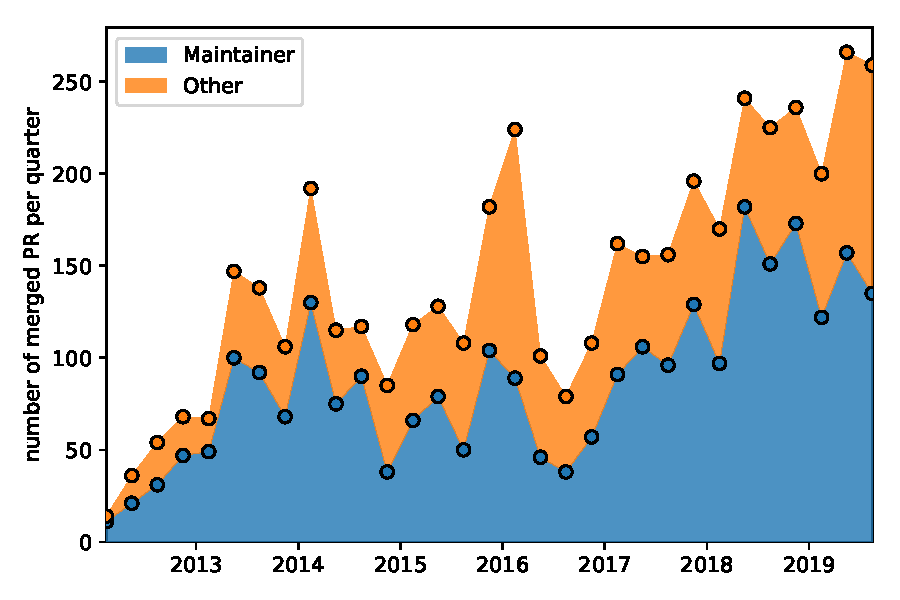
\includegraphics[width=0.9\linewidth]{scripts/PRs-using-CURRENT_MAINTAINERS.pdf}
    \caption{Number of pull requests merged into the NumPy master branch for each
        quarter since 2012. The total number of PRs is indicated with the
        lower blue area showing the portion contributed by current or previous
        maintainers.}\label{fig:prs-over-time}
\end{figure}

NumPy is currently maintained by a group of 23 contributors with commit rights
to the NumPy code base. Out of these, 17 maintainers were active in
2019, 4 of whom were paid to work on the project full-time.
Additionally, there are a few long term developers who contributed and maintain
specific parts of NumPy, but are not officially maintainers.
At a release cycle of about every half year, the five recent releases in the years
2018 and 2019 have averaged about 450~pull requests~(PRs) each,\footnote{
    Note that before mid 2011, NumPy development did not happen on \url{github.com}.
    All data provided here is based on the development which happened through GitHub
    pull requests. In some cases contributions by maintainers may not be categorized as such.}
% Since 1.14.0 (based on changelog): 381 + 438 + 490 + 531 + 402; last is preliminary
with each release attracting more than a hundred new contributors.
Figure~\ref{fig:prs-over-time} shows the number of PRs merged into the NumPy
master branch.
Although the number of PRs being merged fluctuates,
the plot indicates an increased number of contributions over the past
years.

\subsection{Enabling factors}

The creation of NumPy spurred renewed development in the larger scientific
Python ecosystem and heralded the current era of wide-spread use of Python for
scientific computing.
As we implied above, there were several factors that allowed this rapid growth
and successful development.

Hugunin identified the first factor in his initial description of the Numeric
package \cite{Hugunin-whitepaper}.  Numerical computing is usually one
component of a larger programming task.  Therefore:

\begin{quote}
    Rather than trying to retrofit an existing numerical language to support
    the wealth of features found in a powerful, modern, general-purpose
    programming language, it makes much more sense to attack the problem from
    the other direction and add the features of a powerful numerical
    programming language to Python.
\end{quote}

Python is already a good choice for many standard programming tasks such as
cleaning data, interacting with web resources and parsing text.  It has a wide
range of libraries for many different tasks. Adding fast array operations and
linear algebra allows the scientist to do all their work with within the same
language---and one that has the advantage of being famously easy to learn and
teach.

The second factor flows from Python's nature as an open-source language,
embedded within the open-source community.  Python attracts developers who like
to build and contribute.  As a result, NumPy has always been a library that was
developed by scientists in order to do their work.  Commercial specialist
numerical languages can encourage consumer-users, who pick up a tool and use
it, but do not expect to contribute to development.  In contrast, NumPy often
attracts user-developers, who want to work with NumPy, and are prepared to fix
and extend the library as they work. User-developers have been the fundamental
force in developing NumPy, and shaping it into a library that has been refined
in the furnace of practical scientific work.

The third factor is much like the second: a culture in Python that concentrates
on high quality of code and distribution. Because Python is open-source, it has
a strong culture of contribution, and therefore, of using tools and process to
improve collaborative software development, such as distributed version
control, code review, and automated testing.  These have allowed the project to
scale safely as it attracted more users and developers, even though these
developers rarely came to the project with training in software engineering.

Lastly, we believe NumPy has benefited greatly from a well-chosen application
programming interface (API).  Scientific and numerical programming needs to be
fast, and scale to very large datasets.  The NumPy API defines a simple wrapper
for data in memory so it can be represented as a one- or multi-dimensional
array.  The simplicity of this wrapper has made it very successful as a
standard way of representing arrays in memory, and has made it relatively easy
for other libraries to develop fast and memory-efficient compiled code, usually
in C or Fortran, that can manipulate these arrays and pass them back to Python.
This has been a large factor in the growth of numerical computing libraries
around NumPy and Python.

\subsection{Hybrid development}

For many years, NumPy had no dedicated funding, and development time
was mostly contributed freely by students and researchers in their
spare time.  In-person meetings were sponsored off of individual's
research grants, and while industry sponsored contributions were made,
notably those by Mark Wiebe when he was sponsored by Travis Oliphant
at Continuum Analytics, the package's rapid adoption in scientific
computing took place without external investment.

% BIDS -- UCB
% https://www.moore.org/grant-detail?grantId=GBMF5447
% $645,020 in 2016
% https://sloan.org/grant-detail/8222
% $659,359 in 2017
% https://bids.berkeley.edu/news/bids-receives-sloan-foundation-grant-contribute-numpy-development
% http://doi.org/10.5281/zenodo.3585761
% http://doi.org/10.5281/zenodo.3585767
In 2017, NumPy received its first large grants totaling 1.3M USD from the
Gordon \& Betty Moore and the Alfred P. Sloan foundations.
These two grants focus on addressing the technical debt accrued over the years and
on setting in place standards and architecture to encourage more sustainable development.
% CZI -- NumFOCUS/QuanSight
% https://chanzuckerberg.com/eoss/proposals/strengthening-numpys-foundations-growing-beyond-code/
% NumPy and OpenBLAS received $195,000 in 2019
% https://labs.quansight.org/blog/2019/11/numpy-openblas-CZI-grant/
NumPy received a third grant for 200K USD from the Chan Zuckerberg
Initiative at the end of 2019.
This grant focuses on better serving NumPy's large number of beginning
to intermediate level users and on growing the community of NumPy
contributors.
Finally, the project receives around 10K USD annually from Tidelift, which is
typically used to fund documentation writers and website developers.

The first activities organized for the new grants were a development planning
sprint, a weekly community call, and a meeting to write a draft roadmap.
Since the roadmap was meant to represent community consensus on future
development, it was presented for comment at the annual SciPy
conference during a so-called ``Birds of a Feather'' session, attended
by more than 100 people.  One additional meeting was held to discuss
specific enhancements, such as the development of a new data-type
system.  The final roadmap was vetted by the community via online
discussion before being accepted.

\section{The \code{ndarray} data structure}


With its first stable release in October 2006, NumPy unified
the scientific Python community and now underpins almost every library
that does numerical computation, including SciPy\cite{virtanen2019scipy},
pandas\cite{mckinney-proc-scipy-2010}, scikit-learn\cite{pedregosa2011scikit},
and scikit-image\cite{vanderwalt2014scikit}.
NumPy consists of the \code{ndarray}-object along with utility functions that
operate on it.
Because of its inherent simplicity---being a pointer to memory with some
associated meta-data about shape, data-type, and so forth---the NumPy array is
the {\it de facto} exchange format for array data in Python.
The library has such widespread adoption that not only the array object but also its
{\it Application Programming Interface} (API) has become ubiquitous as
a language for tensor computation---witnessed by its use in popular
deep learning libraries such as PyTorch\cite{pytorch}.

The \code{ndarray} data structure stores regularly spaced elements of a single
data type in a contiguous block of memory; along with meta-data such as shape,
it allows for the efficient representation of $n$-dimensional arrays.

\fixme{discuss .. vectors / matrices / and then more ...
indexing and slicing, one-liners that would be tens or hundreds of lines of code in
languages such as C.}

More details about the data structure are given in ``The NumPy array:
a structure for efficient numerical computation.''\cite{vanderwalt2011numpy}.


\begin{lstlisting}
>>> import numpy as np
>>> x = np.array([0, 1, 2, 3])
>>> x.dtype
dtype('int64')
>>> x.shape
(4,)

>>> y = 2 * x
>>> y
array([0, 2, 4, 6])

>>> x * y
array([ 0,  2,  8, 18])

>>> x @ y
28
\end{lstlisting}

\begin{lstlisting}
>>> import numpy as np
>>> x = np.array([1, 2])
>>> A = np.array([[0.1, 0.2], [0.3, 0.2]])
>>> A.dtype 
dtype('float64')
>>> A.shape
(2, 2)

>>> A * x
array([[0.1, 0.4],
       [0.3, 0.4]])

>>> A @ x
array([0.5, 0.7])
>>> x @ A
array([0.7, 0.6])
\end{lstlisting}

NumPy provides a large collection of functions for array manipulation
including functions for: creating, reshaping, concatenating, and padding arrays;
searching, sorting and counting data
in arrays; computing elementary statistics, such as the mean, median,
variance, and standard deviation; file I/O; and more.
It also provides extensive support for generating pseudorandom numbers
as well as an assortment of probability distributions.
For historical reasons, NumPy also includes basic functionality for
linear algebra, fast Fourier transforms and windowing,
and polynomial fitting.
We will continue supporting these, but we will not expand beyond them.

\section{Recent technical improvements}

With the recent infusion of funding and a clear process for coordinating with
the developer community, we have been able to tackle a number of important
large scale changes.
We highlight two of those below.

\subsection{The Array Function Protocol}

A vast number of projects are built on NumPy;
these projects are consumers of the NumPy API.
Over the last several years, a growing number of projects are providers of
a \emph{NumPy-like API} and array objects targeting audiences with specialized
needs beyond NumPy's capabilities.
For example, the NumPy API is implemented by several popular tensor computation
libraries including CuPy\footnote{\url{https://cupy.chainer.org/}},
Jax\footnote{\url{https://jax.readthedocs.io/en/latest/jax.numpy.html}},
PyTorch\footnote{\url{https://pytorch.org/tutorials/beginner/blitz/tensor\_tutorial.html}}, and
and Apache MXNet\footnote{\url{https://mxnet.incubator.apache.org/api/python/docs/api/ndarray/index.html}}.
It is also implemented in packages that support sparse arrays
such as \code{scipy.sparse} and \code{pydata.sparse}.
Another notable example is Dask, a library for parallel computing in
Python.  Dask adopts the NumPy API and therefore presents a familiar
interface to existing NumPy users, while adding powerful abilities to
parallelize and distribute tasks.

The multitude of specialized projects creates the difficulty that consumers
of these NumPy-like APIs write code specific to a single project and do not support
all of the above array providers.
This is a burden for users relying on the specialized array-like, since
a tool they need may not work for them.
It also creates new challenges for end-users who need to transition
from NumPy to a more specialized array.
The growing multitude of specialized projects with NumPy-like APIs threatened
to again fracture the scientific Python community.

To address these issues NumPy has the goal of providing the fundamental
API for \emph{interoperability} between the various NumPy-like APIs.
An earlier step in this direction was the implementation of the
\code{\_\_array\_ufunc\_\_} protocol in NumPy 1.13, which enabled interoperability
for most mathematical functions.\cite{NEP13}
In 2019 this was expanded more generally with the inclusion of the
\code{\_\_array\_function\_\_} protocol into NumPy~1.17.
These two protocols allows providers of array-like APIs to be interoperable
with the NumPy API: their arrays work correctly with almost all NumPy functions.\cite{NEP18}
For the users relying on specialized array projects it means that even though
much code is written specifically for NumPy arrays and uses the NumPy API as
\code{import numpy as np}, it can nevertheless work for them.  For
example, here is how a CuPy GPU array can be passed through NumPy for
processing, with all operations being dispatched back to CuPy:

\begin{lstlisting}
import numpy as np
import cupy as cp

x_gpu = cp.array([1, 2, 3])
y = np.sum(x_gpu)  # Returns a GPU array
\end{lstlisting}

\subsection{Random}

The NumPy random module provides pseudorandom numbers from a wide range of
distributions. In legacy versions of NumPy, simulated random values are produced
by a \code{RandomState} object that: handles seeding and state initialization;
wraps the core pseudorandom number generator based on a 32-bit implementation of
MT19937; interfaces with the underlying code that transforms random bits into
deviates from other distributions; and supplies a singleton instance exposed in
the root of the random module.

The \code{RandomState} object makes a compatibility guarantee so that a fixed
seed and sequence of function calls produce the same set of values. This
guarantee has slowed progress since improving the underlying code requires
extending the API with additional keyword arguments. This guarantee continues to
apply to \code{RandomState}. 

NumPy 1.17 introduced a new API for generating random numbers that use a more
flexible structure that can be extended by libraries or end-users. The new API
is built using components that separate the steps required to generate random
variates. Pseudorandom bits are generated by a bit generator. These bits are
then transformed into variates from complex distributions by a generator.
Finally, seeding is handled by an object that produces sequences of high-quality
initial values.

Bit generators are simple classes that manage the state of an underlying
pseudorandom number generator. NumPy ships with four bit generators. The default
bit generator is a 64-bit implementation of the Permuted Congruential Generator
\cite{pcg64} (\code{PCG64}). The three other bit generators are a 64-bit version
of the Philox generator\cite{random123} (\code{Philox}), Chris Doty-Humphrey's
Small Fast Chaotic generator\cite{practrand} (\code{SFC64}), and the 32-bit
Mersenne Twister\cite{mt19937} (\code{MT19937}) which has been used in older
versions of NumPy.\footnote{The
\href{https://github.com/bashtage/randomgen}{randomgen project} supplies a wide
range of alternative bit generators such as a cryptographic counter-based
generators (\code{AESCtr}) and generators that expose hardware random number
generators (\code{RDRAND})\cite{randomgen}.} Bit generators export a capsule
containing pointers to functions that produce 64 bits, 32 bits, or a random
double. They also expose CFFI and ctypes interfaces to the same three functions.

The \code{Generator} consumes one of the bit generators and produces variates
from complicated distributions. Many improved methods for generating random
variates from common distributions were implemented, including the Ziggurat
method for normal, exponential and gamma variates\cite{ziggurat}, and Lemire's
method for bounded random integer generation\cite{lemire}. The \code{Generator}
is more similar to the legacy \code{RandomState}, and its API is substantially
the same. The key differences all relate to state management, which has been
delegated to the bit generator. The \code{Generator} does not make the same
stream guarantee as the \code{RandomState} object, and so variates may differ
across versions as improved generation algorithms are
introduced.\footnote{Despite the removal of the compatibility guarantee, simple
reproducibility across versions is encouraged, and minor changes that do not
produce meaningful performance gains or fix underlying bug are not generally
adopted.}

Finally, a \code{SeedSequence} is used to initialize a bit generator. The seed
sequence can be initialized with no arguments, in which case it reads entropy
from a system-dependent provider, or with a user-provided seed. The seed
sequence then transforms the initial set of entropy into a sequence of
high-quality pseudorandom integers, which can be used to initialize multiple bit
generators deterministically. A key design goal of a seed sequence was to be
splittable in the sense that a seed sequence can be used to produce child
sequences that are distinct from their parents or other ancestors. This
capability allows a seed sequence to be used in large distributed applications
where the number of workers required is not known. The sequences generated from
the same initial entropy and the same splits are fully deterministic to ensure
reproducibility.

The three components are combined to construct a complete random number
generator.

\begin{lstlisting}
from numpy.random import (
    Generator,
    PCG64,
    SeedSequence,
)

seq = SeedSequence(1030424547444117993331016959)
pcg = PCG64(seq)
gen = Generator(pcg)
\end{lstlisting}

\noindent This approach retains access to the seed sequence which can then be
used to spawn additional generators.

\begin{lstlisting}
children = seq.spawn(2)
gen_0 = Generator(PCG64(children[0]))
gen_1 = Generator(PCG64(children[1]))
\end{lstlisting}

\noindent While this approach retains complete flexibility, the method
\code{np.random.default\_rng} can be used to instantiate a \code{Generator} when
reproducibility is not needed.

The final goal of the new API is to improve extensibility. \code{RandomState} is
a monolithic object that obscures all of the underlying state and functions. The
component architecture is one part of the extensibility improvements. The
underlying functions (written in C) which transform the output of a bit
generator to other distributions are available for use in CFFI. This allows the
same code to be run in both NumPy and dependent that can consume CFFI, e.g.,
Numba. Both the bit generators and the low-level functions can also be used in C
or Cython code.\footnote{As of 1.18.0, this scenario requires access to the
NumPy source. Alternative approaches that avoid this extra step are being
explored.} 

\section{Discussion}

% 1st grant done, technical cleanup finished except dtypes
% 2nd grant starting, community growth and new user focus

Most of the technical work for the Moore and Sloan grant is now complete.
The main remaining item is an overhaul of the data type system, which
we are currently working on.
The meaning of each element within a NumPy array is described by its
datatype (dtype). NumPy arrays can hold all common numerical
datatypes, strings, datetimes, and generic Python objects, each of
which is identified by a dtype.
%We are busy overhauling the datatype
%system to make it behave consistently and to simplify the creation of
%custom dtypes, both in C and in Python [XXX Cite the NEP here, instead
%of \href{https://github.com/numpy/numpy/pull/14422}{draft of DTypes NEP}].
While numerical dtypes make the foundation for most users,
there are a multitude of use cases which cannot prosper due to current
limitations, such as physical units\cite{astropy,Goldbaum2018,pint},
% pyadolc may be a bit too small a project, so may want to remove/replace with an other example.
geometrical objects\cite{pygeos}, and automatic
differentiation\cite{pyadolc}.
%Projects addressing these exist, each struggles with current
%limitations.  % TODO: I may need citations, we could link github issues.
The proposed overhaul of the datatype system will make it behave consistently and
to simplify the creation of custom dtypes, both in C and in Python

%% While it is currently possible to define custom dtypes within NumPy, many of the
%% use cases above cannot be solved using this system.
%% This is evidenced also by code within NumPy which would require changes
%% in many places to add such dtypes, even when adding them within NumPy itself.
%% The new implementation will be simpler and more cleanly implemented in
%% this regard.
%% Custom dtypes and the basic dtypes included within NumPy will be implemented
%% and behave identically as much as possible.
%% At the same time redesigning the API will make NumPy dtypes more flexible to grow
%% to future needs should they arise.

%% As a further step, to make dtypes more accessible and allow a faster adoption of
%% custom dtypes within the community, we plan to create a Python API to
%% define such custom dtypes.

Having made progress on addressing technical debt accrued over two decades of
development and modernizing the code to handle new use cases, the project
is ready to grow its community of contributors and to better address the needs
of an ever-growing number of new users.  This is the main focus of the
forthcoming CZI grant.

[... CZI grant ...]

[... welcome new users ...]

% technical focus
% improve various aspects of NumPy, including easier construction of custom data types (e.g., missing values, physical units, times & dates) and better integration with arrays customized for specialized domains (e.g., SciPy's sparse arrays, pandas' DataFrames, and xarray's labeled arrays). 
% technical work, and it increased the velocity of the projects by ~25-30%, and in addition it enabled integrating some larger changes, like the numpy.random redesign.


% \subsubsection*{Future Development}

% Dtypes

% outline plan for the CZI grant and an invitation to new contributors

%\subsection*{Website}


\bibliography{references}

\newpage

We use Git for version control and GitHub as the public hosting service for our
official \emph{upstream} repository (\url{https://github.com/numpy/numpy}).
We each work in our own copy (or fork) of the project and use the
upstream repository as our integration point.
To get new code into the upstream repository, we use GitHub's
pull request (PR) mechanism.
This allows us to review code before integrating it as well as to run a
large number of tests on the modified code to ensure that the changes
do not break expected behavior.

We also use GitHub's issue tracking system to collect and triage problems and
proposed improvements.


\section*{Library organization}

Broadly, the NumPy library consists of the following parts:
the NumPy array data structure \texttt{ndarray}; the so-called \emph{universal functions};
a set of library functions for manipulating arrays and doing scientific
computation; infrastructure libraries for unit tests and Python package
building; and the program \texttt{f2py} for wrapping Fortran code in Python \cite{peterson2009f2py}.
The \texttt{ndarray} and the universal functions are generally considered
the core of the library.
In the following, we give a brief summary of these components of the
library.

\subsection*{Core}

The \texttt{ndarray} data structure and the
universal functions make up the core of NumPy.

The \texttt{ndarray} is the data structure at the heart of NumPy.
The data structure stores regularly strided homogeneous data types
inside a contiguous block memory, allowing for the efficient representation
of $n$-dimensional data.
More details about the data structure are given in ``The NumPy array:
a structure for efficient numerical computation'' \cite{vanderwalt2011numpy}.

The \emph{universal functions}, or more concisely, \emph{ufuncs},
are functions written in C that implement efficient looping over
NumPy arrays. An important feature of ufuncs is the built-in
implementation of \emph{broadcasting}.  For example, the function
\texttt{arctan2(x, y)} is a ufunc that accepts two values and computes
$\tan^{-1}(y/x)$.  When arrays are passed in as the arguments,
the ufunc will take care of looping over the dimensions of the inputs
in such a way that if, say, \texttt{x} is a 1-D array with length 3, and
\texttt{y} is a 2-D array with shape $2 \times 1$, the output will be
an array with shape $2 \times 3$ (Fig.~\ref{fig:array-concepts}c).
The ufunc machinery takes care
of calling the function with all the appropriate combinations of
input array elements to complete the output array.
The elementary arithmetic operations of addition, multiplication, etc.,
are implemented as ufuncs, so that broadcasting also applies to expressions
such as \texttt{x + y * z}.

\subsection*{Computing libraries.}

NumPy provides a large library of functions for array manipulation
and scientific computing, including functions for: creating, reshaping,
concatenating, and padding arrays; searching, sorting and counting data
in arrays; computing elementary statistics, such as the mean, median,
variance, and standard deviation; file I/O; and more.

NumPy's linear algebra library provides an interface to established
linear algebra methods. These include solving linear systems of equations
and computing various matrix properties, such as the determinant,
the norm, the inverse, and the pseudo-inverse.
As well as computing the Cholesky, eigenvalue, and singular value decompositions
of a matrix and further functions.
For best performance and reliability the algorithms are provided by leveraging
an external implementation of the LAPACK interface \cite{LAPACK}.
LAPACK itself was first released in 1992 and is based on the EISPACK and LINPACK
open-source libraries. It is part of Netlib, a repository of
mathematical software, papers and databases and has a long history of open,
community-wide development \cite{dongarra1990lapack,dongarra2008netlib}.

The random number generator library in NumPy provides alternative
\emph{bit stream generators} that provide the core function of generating
random integers.
A higher-level generator class that implements an assortment of
probability distributions is provided. It includes the beta, gamma
and Weibull distributions, the univariate and multivariate normal
distributions, and more.

A suite of functions for computing the \emph{fast Fourier transform (FFT)}
and its inverse is provided.

\subsection*{Infrastructure libraries}

NumPy provides utilities for writing tests and for building Python packages.

The \texttt{testing} subpackage provides functions such as
\texttt{assert\_allclose(actual, desired)} that may be used in
test suites for code that uses NumPy arrays.

NumPy provides the subpackage \texttt{distutils} which includes functions and classes
to facilitate configuration, installation, and packaging of libraries depending on NumPy.
% Remove the PyPI reference entirely?
These can be used, for example, when publishing to the PyPI website.

\subsection*{F2PY}  The program \texttt{f2py} is a tool for
building NumPy-aware Python wrappers of Fortran functions.
NumPy itself does not use any Fortran code;  F2PY is part of NumPy
for historical reasons.


\section*{Governance}

% https://mail.python.org/pipermail/numpy-discussion/2015-October/073849.html
% https://github.com/numpy/numpy/pull/6352
NumPy adopted an official Governance Document on October~5,
2015 (\url{https://numpy.org/devdocs/dev/governance/governance.html}).
Project decisions are usually made by consensus of interested contributors.
This means that, for most decisions, everyone is entrusted with veto power.
A Steering Council, currently composed of 12~members, facilitates this
process and oversees daily development of the project by contributing code
and reviewing contributions from the community.

% https://mail.python.org/pipermail/numpy-discussion/2018-July/078476.html
% https://github.com/numpy/numpy/pull/11865
NumPy's official Code of Conduct was approved on September~1, 2018
(\url{https://numpy.org/devdocs/dev/conduct/code_of_conduct.html}).
In brief, we strive to:
\emph{be open};
\emph{be empathetic, welcoming, friendly, and patient};
\emph{be collaborative};
\emph{be inquisitive}; and
\emph{be careful in the words that we choose}.
The Code of Conduct also specifies how breaches can be reported and outlines
the process for responding to such reports.

\section*{Funding}

% BIDS -- UCB
% https://www.moore.org/grant-detail?grantId=GBMF5447
% $645,020 in 2016
% https://sloan.org/grant-detail/8222
% $659,359 in 2017
% https://bids.berkeley.edu/news/bids-receives-sloan-foundation-grant-contribute-numpy-development
% http://doi.org/10.5281/zenodo.3585761
% http://doi.org/10.5281/zenodo.3585767
In 2017, NumPy received its first large grants totaling 1.3M USD from the
Gordon \& Betty Moore and the Alfred P. Sloan foundations.
Stéfan van der Walt is the PI and manages four programmers working on the project.
These two grants focus on addressing the technical debt accrued over the years and
on setting in place standards and architecture to encourage more sustainable development.

% CZI -- NumFOCUS/QuanSight
% https://chanzuckerberg.com/eoss/proposals/strengthening-numpys-foundations-growing-beyond-code/
% NumPy and OpenBLAS received $195,000 in 2019
% https://labs.quansight.org/blog/2019/11/numpy-openblas-CZI-grant/
NumPy received a third grant for 195K USD from the Chan Zuckerberg
Initiative at the end of 2019 with Ralf Gommers as the PI.
This grant focuses on better serving NumPy's large number of beginning
to intermediate level users and on growing the community of NumPy
contributors.
It will also provide support to OpenBLAS, on which NumPy depends for
accelerated linear algebra.

Finally, since May 2019 the project receives a small amount annually from
Tidelift, which is used to fund things like documentation and website
improvements.


\section*{Developers}

NumPy is currently maintained by a group of 23 contributors with commit rights
to the NumPy code base. Out of these, 17 maintainers were active in
2019, 4 of whom were paid to work on the project full-time.
Additionally, there are a few long term developers who contributed and maintain
specific parts of NumPy, but are not officially maintainers.

Over the course of its history, NumPy has attracted PRs by 823 contributors.
However, its development relies heavily on a small number
of active maintainers, who share more than half of the contributions among
themselves.

At a release cycle of about every half year, the five recent releases in the years
2018 and 2019 have averaged about 450~PRs each,\footnote{
    Note that before mid 2011, NumPy development did not happen on \url{github.com}.
    All data provided here is based on the development which happened through GitHub
    PRs. In some cases contributions by maintainers may not be categorized as such.}
% Since 1.14.0 (based on changelog): 381 + 438 + 490 + 531 + 402; last is preliminary
with each release attracting more than a hundred new contributors.
Figure~\ref{fig:prs-over-time} shows the number of PRs merged into the NumPy
master branch.
Although the number of PRs being merged fluctuates,
the plot indicates an increased number of contributions over the past
years.

\begin{figure}
    \centering
    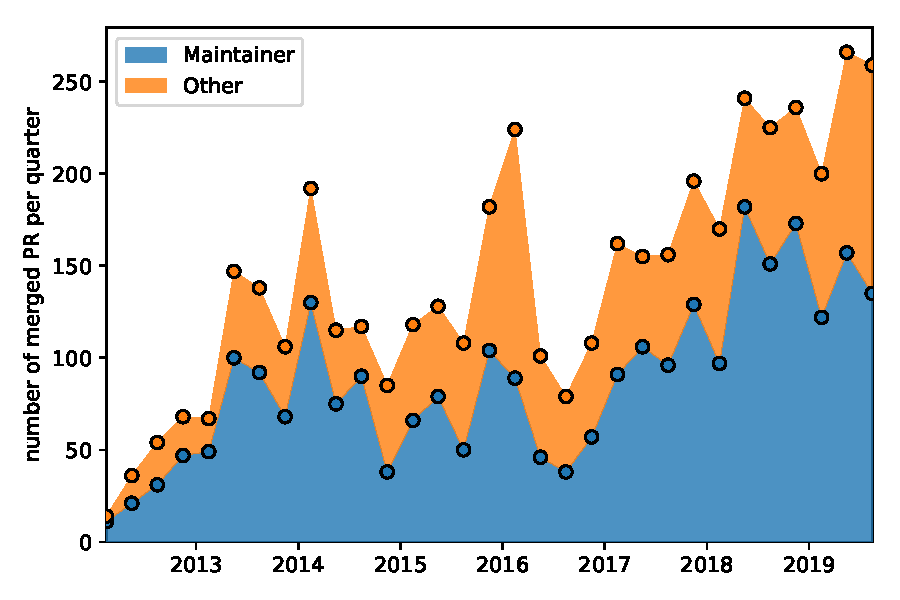
\includegraphics[width=0.9\linewidth]{scripts/PRs-using-CURRENT_MAINTAINERS.pdf}
    \caption{\textbf{Number of pull requests merged into the NumPy master branch for each
        quarter since 2012.} The total number of PRs is indicated with the
        lower blue area showing the portion contributed by current or previous
        maintainers.}\label{fig:prs-over-time}
\end{figure}



\section*{Community calls}

The massive number of scientific Python packages that
built on NumPy meant that it had an unusually high need for stability.
So to guide our development we formalized the feature proposal process, and
constructed a development roadmap with extensive input and feedback from the
community.


Weekly community calls alternate between triage and
higher level discussion.  The calls not only involve developers from
the community, but provide a venue for vendors and other external
groups to provide input.  For example, after Intel produced a forked
version of NumPy, one of their developers joined a call to discuss
community concerns.

\section*{NumPy enhancement proposals}

Given the complexity of the codebase and the massive number of projects depending
on it, large changes require careful planning and substantial work.
NumPy Enhancement Proposals (NEPs) are modeled after
Python Enhancement Proposals (PEPs) for ``proposing major new
features, for collecting community input on an issue, and for
documenting the design decisions that have gone into
Python''\footnote{\url{https://numpy.org/neps/nep-0000.html}}.
Since then there have been 19 proposed NEPS---6 have been implemented,
4 have been accepted and are being implemented, 4 are under
consideration, 3 have been deferred or superseded, and 2 have been rejected
or withdrawn.


\section*{Central role}

NumPy plays a central role in building and standardizing much of the scientific
Python community infrastructure.
NumPy's docstring standard is now widely adopted.
We are also now using the NEP system as a way to help coordinate the larger
scientific Python community.
% https://numpy.org/neps/nep-0029-deprecation_policy.html
For example, in NEP 29, we recommend, along with leaders from various other
projects, that all projects across the Scientific Python ecosystem adopt a
common ``time window-based'' policy for support of Python and NumPy versions.
This standard will simplify downstream project and release planning.

\section*{Wheels build system}

A Python \emph{wheel} (\url{https://www.python.org/dev/peps/pep-0427/})
is a standard file format for distributing Python libraries.
In addition to Python code, a wheel may include compiled
C extensions and other binary data.
This is important, because many libraries, including NumPy,
require a C compiler and other build tools to build the software
from the source code, making it difficult for many users to install
the software on their own.  The introduction of wheels to the Python
packaging system has made it much easier for users to install
precompiled libraries.

A GitHub repository containing scripts to build NumPy wheels has
been configured so that a simple commit to the repository triggers
an automated build system that creates NumPy wheels for several
computer platforms, including Windows, Mac OSX and Linux.  The wheels
are uploaded to a public server and made available for anyone to use.
This system makes it easy for users to install precompiled versions
of NumPy on these platforms.

The technology that is used to build the wheels evolves continually.
At the time this paper is being written, a key component is the
\texttt{multibuild} suite of tools developed by Matthew Brett and
other developers (\url{https://github.com/matthew-brett/multibuild}).
Currently, scripts using \texttt{multibuild} are written for
the continuous integration platforms Travis-CI (for Linux and Mac OSX)
and Appveyor (for Windows).

\section*{Recent technical improvements}

With the recent infusion of funding and a clear process for coordinating with
the developer community, we have been able to tackle a number of important
large scale changes.
We highlight two of those below, as well as changes made to our testing
infrastructure to support hardware platforms used in large scale computing.

\section*{Array function protocol}

A vast number of projects are built on NumPy;
these projects are consumers of the NumPy API.
Over the last several years, a growing number of projects are providers of
a \emph{NumPy-like API} and array objects targeting audiences with specialized
needs beyond NumPy's capabilities.
For example, the NumPy API is implemented by several popular tensor computation
libraries including CuPy\footnote{\url{https://cupy.chainer.org/}},
JAX\footnote{\url{https://jax.readthedocs.io/en/latest/jax.numpy.html}},
and Apache MXNet\footnote{\url{https://numpy.mxnet.io/}}.
PyTorch\footnote{\url{https://pytorch.org/tutorials/beginner/blitz/tensor\_tutorial.html}}
and Tensorflow\footnote{\url{https://www.tensorflow.org/tutorials/customization/basics}}
provide tensor APIs with NumPy-inspired semantics.
It is also implemented in packages that support sparse arrays
such as \texttt{scipy.sparse} and PyData/Sparse.
Another notable example is Dask, a library for parallel computing in
Python.  Dask adopts the NumPy API and therefore presents a familiar
interface to existing NumPy users, while adding powerful abilities to
parallelize and distribute tasks.

The multitude of specialized projects creates the difficulty that consumers
of these NumPy-like APIs write code specific to a single project and do not support
all of the above array providers.
This is a burden for users relying on the specialized array-like, since
a tool they need may not work for them.
It also creates challenges for end-users who need to transition
from NumPy to a more specialized array.
The growing multitude of specialized projects with NumPy-like APIs threatened
to again fracture the scientific Python community.

To address these issues NumPy has the goal of providing the fundamental
API for \emph{interoperability} between the various NumPy-like APIs.
An earlier step in this direction was the implementation of the
\texttt{\_\_array\_ufunc\_\_} protocol in NumPy 1.13, which enabled interoperability
for most mathematical functions (\url{https://numpy.org/neps/nep-0013-ufunc-overrides.html}).
In 2019 this was expanded more generally with the inclusion of the
\texttt{\_\_array\_function\_\_} protocol into NumPy~1.17.
These two protocols allow providers of array objects to be interoperable
with the NumPy API: their arrays work correctly with almost all NumPy
functions (\url{https://numpy.org/neps/nep-0018-array-function-protocol.html}).
For the users relying on specialized array projects it means that even though
much code is written specifically for NumPy arrays and uses the NumPy API as
\texttt{import numpy as np}, it can nevertheless work for them.
For example, here is how a CuPy GPU array can be passed through NumPy for
processing, with all operations being dispatched back to CuPy:

\begin{lstlisting}
import numpy as np
import cupy as cp

x_gpu = cp.array([1, 2, 3])
y = np.sum(x_gpu)  # Returns a GPU array
\end{lstlisting}

Similarly, user defined functions composed using NumPy can now be
applied to, e.g., multi-node distributed Dask arrays:

\begin{lstlisting}
import numpy as np
import dask.array as da


def f(x):
    """Function using NumPy API calls"""
    y = np.tensordot(x, x.T)
    return np.mean(np.log(y + 1))


x_local = np.random.random([10000, 10000])  # random local array
x_distr = da.random.random([10000, 10000])  # random distributed array

f(x_local)  # returns a NumPy array
f(x_distr)  # works, returns a Dask array
\end{lstlisting}

\section*{Random number generation}

The NumPy \texttt{random} module provides pseudorandom numbers from a wide range of
distributions. In legacy versions of NumPy, simulated random values are produced
by a \texttt{RandomState} object that: handles seeding and state initialization;
wraps the core pseudorandom number generator based on a Mersenne Twister
implementation\footnote{to be precise, the standard 32-bit version of MT19937};
interfaces with the underlying code that transforms random bits into
variates from other distributions; and supplies a singleton instance exposed in
the root of the random module.

The \texttt{RandomState} object makes a compatibility guarantee so that a fixed
seed and sequence of function calls produce the same set of values. This
guarantee has slowed progress since improving the underlying code requires
extending the API with additional keyword arguments. This guarantee continues to
apply to \texttt{RandomState}.

NumPy 1.17 introduced a new API for generating random numbers that use a more
flexible structure that can be extended by libraries or end-users. The new API
is built using components that separate the steps required to generate random
variates. Pseudorandom bits are generated by a bit generator. These bits are
then transformed into variates from complex distributions by a generator.
Finally, seeding is handled by an object that produces sequences of high-quality
initial values.

Bit generators are simple classes that manage the state of an underlying
pseudorandom number generator. NumPy ships with four bit generators. The default
bit generator is a 64-bit implementation of the Permuted Congruential Generator
\cite{pcg64} (\texttt{PCG64}). The three other bit generators are a 64-bit version
of the Philox generator \cite{random123} (\texttt{Philox}), Chris Doty-Humphrey's
Small Fast Chaotic generator \cite{practrand} (\texttt{SFC64}), and the 32-bit
Mersenne Twister \cite{mt19937} (\texttt{MT19937}) which has been used in older
versions of NumPy.\footnote{The
\href{https://github.com/bashtage/randomgen}{randomgen project} supplies a wide
range of alternative bit generators such as a cryptographic counter-based
generators (\texttt{AESCtr}) and generators that expose hardware random number
generators (\texttt{RDRAND}) \cite{randomgen}.} Bit generators provide
functions, exposed both in Python and C, for generating random integer
and floating point numbers. The three new bit generators were chosen for their
combination of statistical soundness and performance. The PCG family of generators
have been widely tested using state-of-the-art statistical tests and found to
perform well \cite{lemire_blog}. All three of the new generators were tested
using the PractRand test suite \cite{practrand} with four TB of random values.
Each was tested using a single generator and using a composite generator assembled
from multiple copies of the same bit generator, each seeded from a shared
\texttt{SeedSequence}.

The \texttt{Generator} consumes one of the bit generators and produces variates
from complicated distributions. Many improved methods for generating random
variates from common distributions were implemented, including the Ziggurat
method for normal, exponential and gamma variates \cite{ziggurat}, and Lemire's
method for bounded random integer generation \cite{lemire}. The \texttt{Generator}
is more similar to the legacy \texttt{RandomState}, and its API is substantially
the same. The key differences all relate to state management, which has been
delegated to the bit generator. The \texttt{Generator} does not make the same
stream guarantee as the \texttt{RandomState} object, and so variates may differ
across versions as improved generation algorithms are
introduced.\footnote{Despite the removal of the compatibility guarantee, simple
reproducibility across versions is encouraged, and minor changes that do not
produce meaningful performance gains or fix underlying bug are not generally
adopted.}

Finally, a \texttt{SeedSequence} is used to initialize a bit generator. The seed
sequence can be initialized with no arguments, in which case it reads entropy
from a system-dependent provider, or with a user-provided seed. The seed
sequence then transforms the initial set of entropy into a sequence of
high-quality pseudorandom integers, which can be used to initialize multiple bit
generators deterministically. The key feature of a seed sequence is that
it can be used to spawn child \texttt{SeedSequence}s to initialize
multiple distinct bit generators.
% Of course there is a diminishing chance of collisions...
% Only found http://www.pcg-random.org/posts/developing-a-seed_seq-alternative.html
% as a reference for seed sequence, it would be nice to cite something.
This capability allows a seed sequence to facilitate large distributed applications
where the number of workers required is not known. The sequences generated from
the same initial entropy and spawns are fully deterministic to ensure
reproducibility.

The three components are combined to construct a complete random number
generator.

\begin{lstlisting}
from numpy.random import (
    Generator,
    PCG64,
    SeedSequence,
)

seq = SeedSequence(1030424547444117993331016959)
pcg = PCG64(seq)
gen = Generator(pcg)
\end{lstlisting}

This approach retains access to the seed sequence which can then be
used to spawn additional generators.

\begin{lstlisting}
children = seq.spawn(2)
gen_0 = Generator(PCG64(children[0]))
gen_1 = Generator(PCG64(children[1]))
\end{lstlisting}

While this approach retains complete flexibility, the method
\texttt{np.random.default\_rng} can be used to instantiate a \texttt{Generator} when
reproducibility is not needed.

The final goal of the new API is to improve extensibility. \texttt{RandomState} is
a monolithic object that obscures all of the underlying state and functions. The
component architecture is one part of the extensibility improvements. The
underlying functions (written in C) which transform the output of a bit
generator to other distributions are available for use in CFFI. This allows the
same code to be run in both NumPy and dependent that can consume CFFI, e.g.,
Numba. Both the bit generators and the low-level functions can also be used in C
or Cython code.\footnote{As of 1.18.0, this scenario requires access to the
NumPy source. Alternative approaches that avoid this extra step are being
explored.}

\section*{Testing on multiple architectures}

At the time of writing the two fastest supercomputers in the
world, Summit and Sierra, both have IBM POWER9 architectures
(\url{https://www.top500.org/lists/2019/11/}).
In late 2018, Astra, the first ARM-based supercomputer
to enter the TOP500 list, went into production
(\url{https://en.wikichip.org/wiki/supercomputers/astra}).
Furthermore, over 100 billion ARM processors have been produced as
of 2017 (\url{https://en.wikipedia.org/wiki/ARM_architecture}),
making it the most widely used instruction set architecture
in the world.

Clearly there are motivations for a large scientific computing
software library to support POWER and ARM architectures. We've extended
our continuous integration (CI) testing to include \texttt{ppc64le}
(POWER8 on Travis CI) and ARMv8 (on Shippable service). We also test
with the s390x architecture (IBM Z CPUs on Travis CI) so that we
can probe the behavior of our library on a big-endian machine.
This satisfies one of the major components of
improved CI testing laid out in a version of our
roadmap---specifically, ``CI for more exotic
platforms."

PEP 599 (\url{https://www.python.org/dev/peps/pep-0599/})
lays out a plan for new Python binary wheel
distribution support, \texttt{manylinux2014}, that adds
support for a number of architectures supported by the CentOS
Alternative Architecture Special Interest Group, including
ARMv8, ppc64le, as well as s390x. We are thus well-positioned
for a future where provision of binaries on these architectures
will be expected for a library at the base of the ecosystem.


\section*{Acknowledgments}

S.J.v.d.W and K.J.M. were funded in part by the Gordon and Betty Moore
Foundation through Grant GBMF3834 and by the Alfred P. Sloan Foundation through
Grant 2013-10-27 to the University of California, Berkeley.
S.J.v.d.W, S.B., T.J.R., and W.W. were funded in part by the Gordon
and Betty Moore Foundation through Grant GBMF5447 and by the Alfred
P. Sloan Foundation through Grant G-2017-9960 to the University of
California, Berkeley.

We would also like to thank the many members of the community who have provided
feedback, submitted bug reports, made minor improvements to the documentation,
code, or website, promoted its use in their scientific fields, and built
the vast ecosystem of tools and libraries around NumPy.

\section*{Author Contributions Statement}

%C.R.H and T.E.O.
K.J.M. and S.J.v.d.W composed the manuscript with input from others.
S.B., K.S., T.J.R., W.W., and M.B. drafted sections.
All authors have contributed significant code, documentation, and/or expertise
to the NumPy project.
All authors reviewed the manuscript.

\section*{Competing Interests}

The authors declare no competing interests.

\end{document}
